\chapter{\textit{}Structural Risk Minimization}
\label{ch:structuralriskminimization}\index{structuralriskminimization}


\section Overview \newline \index{overview}

Structural Risk Minimization (SRM) is a technique first developed by Vapnik \& Chervonenkis in their book from 1974  \cite{vapnikchervonenkis1}. This technique is used to identify the function $f(x)$ that solves our machine learning problem $y=f(x)$. SRM attempts to find a balance between training our model accurately, and not having an overly complex solution.

Consider the equation below, as shown in \cite{srmvapnik512}:

\begin{equation}\label{srm1}
\centering
\[\underset{f}{min}\left[\hat{R}(f)+\epsilon(f)\right]\]
\end{equation}

The first part of this equation is the training loss, or what we can refer to as the expected risk $\hat{R}(f)$. The expected risk is found based on the training data, and represents the frequency of errors on our training set. Parameters are adjusted to minimize $\hat{R}(f)$ so as to obtain the best possible model for our problem. This technique is referred to as Empirical Risk Minimization (ERM). The second part of the equation $\epsilon(f)$ refers to the capacity measure of the function. This is used to quantify the complexity of our function $f$.

\section VC-Dimension \newline \index{vcdimension}

A vital topic for one to be able to understand SRM is the VC-Dimension. The theory about uniform convergence of empirical risk to actual risk describes various conditions, as well as the bounds for the rate of convergence. These bounds are based upon a measure of the capacity of the set of functions implemented by the model, also known as the VC-Dimension \cite{srmvapnik506}. 


\textbf{Definition}: Given a collection $F$ of subsets of a set $S$, we say that the finite subset $A$ of $S$ is shattered provided that every subset $B$ contained in $A$ can be written as intersection of $A$ with an element of $F$. \cite{vcdbhaskar}


Vapnik \cite{srmvapnik506} defines the VC-Dimension for a set of indicator functions as the maximum number $h$ of vectors that can be shattered in $2^{h}$ ways by using functions within that set. It should be noted that a VC-Dimension of $h$ does not mean that all set of $h$ points can be shattered by a given set of functions, but there is at least one instance of it occurring.


\section Structural Risk Minimization \newline \index{structuralriskminimizationsub}

Suppose $l$ is the size of our sample, and $h$ is our VC dimension. When $\frac{l}{h}$ is large enough, our VC confidence is negligible and hence, it can be ignored and ERM can take place. However, when $\frac{l}{h}$ is small, the VC confidence can no longer be ignored. When this is the case, we need to be able adjust the VC-dimension $h$ of our model \cite{srmvapnik506}. This is where Structural Risk Minimization comes in. It is a technique that allows a tradeoff in accurate model fitting and avoiding overcomplexity. One may think that we would want our VC-dimension $h$ to be a high value, as our risk $R(f)$ drops. However, while this is true, this would increase the chances of overfitting. This is why we have our complexity term $\epsilon$, that increases when this occurs. On the other hand, if $h$ is too low, then we would have an issue of our $R(f)$ being too high. So the user must have the right balance of accuracy and complexity.


In mathematical terms, SRM is carried out by first selecting a family of classifiers $\{F(x,w)\}$, and then defining a structure of nested subsets of the elements of the family: $S_{1}\subset S_{2}\subset\ldots\subset S_{n-1}\subset S_{n}$, where $S_{i}=\left\{ f(x,w),\:w\in W_{i}\right\} $. Due to the structure of the subsets, their respective VC-dimension satisfies: $h_{1}<h_{2}<\ldots<h_{n-1}<h_{n}$. Our goal is to find the optimal structure for our problem, denoted $S^{*}$.


To find this optimal structure, we carry out the following steps, as described by Vapnik in \cite{srmvapnik506} and in \cite{srmkrishnamurthy, srmsewell}:

\begin{enumerate}
\item Find the ERM for each element of the structure $\hat{f_{i}}=arg\,\underset{f\in S_{i}}{min}\hat{R}(f)$
\item Next we calculate $i_{*}=arg\,\underset{i\in\mathbb{N}}{min}R(\hat{f_{i}})+\epsilon_{i}$ and return $f_{i_{*}}$
\end{enumerate}


The following lemma and theorem that provide the mathematical framework for the SRM procedure are shown below, as explained in \cite{srmkrishnamurthy}:

\textbf{Lemma}: For every $\delta\in(0,1)$ and distribution $D$, with probability at least $1-\delta$, the following bounds holds $\forall\:i\in\mathbb{N},\,f\in S_{i}$\:
\begin{equation}\label{lem}
\centering
\left|R(f)-\hat{R}(f)\right|\leq\epsilon_{i}(n,w(i)\delta)\]
\end{equation}

where $\epsilon_{i}(n,w(i)\delta)=min\left\{ \epsilon\,|\,n_{S_{i}}^{UC}(\epsilon,\delta)\leq n\right\} $ is the smallest error achievable in the uniform convergence bound, with $n$ samples and failure probability $\delta$ and $w\colon\mbox{\ensuremath{\mathbb{N}}}\rightarrow\left[0,1\right]$ is the weighting function such that $\underset{i}{\Sigma}w(i)\leq1$.


\textbf{Theorem}: For any $\delta$ and distribution $D$, with probability at least $1-\delta$ the output of the SRM procedure satisfies 
\begin{equation}\label{thm}
\centering
\[R(\hat{f_{i}})\leq\underset{k\in\mathbb{N}}{min}\left\{ \underset{f\in S_{k}}{min}R(f)+2\epsilon_{k}\left(n,w(k)\delta\right)\right\} \]
\end{equation}

Due to sampling issues, if the algorithm were to select the set $S_{i}$ with the lowest true error bound, it could technically return different sets each time. For this reason we use the above theorem that tells us that we can guarantee nearly the same bound as would apply on the smallest set containing our output $f$. 


Below is a diagram illustrating SRM:

\begin{figure*}
\centering
	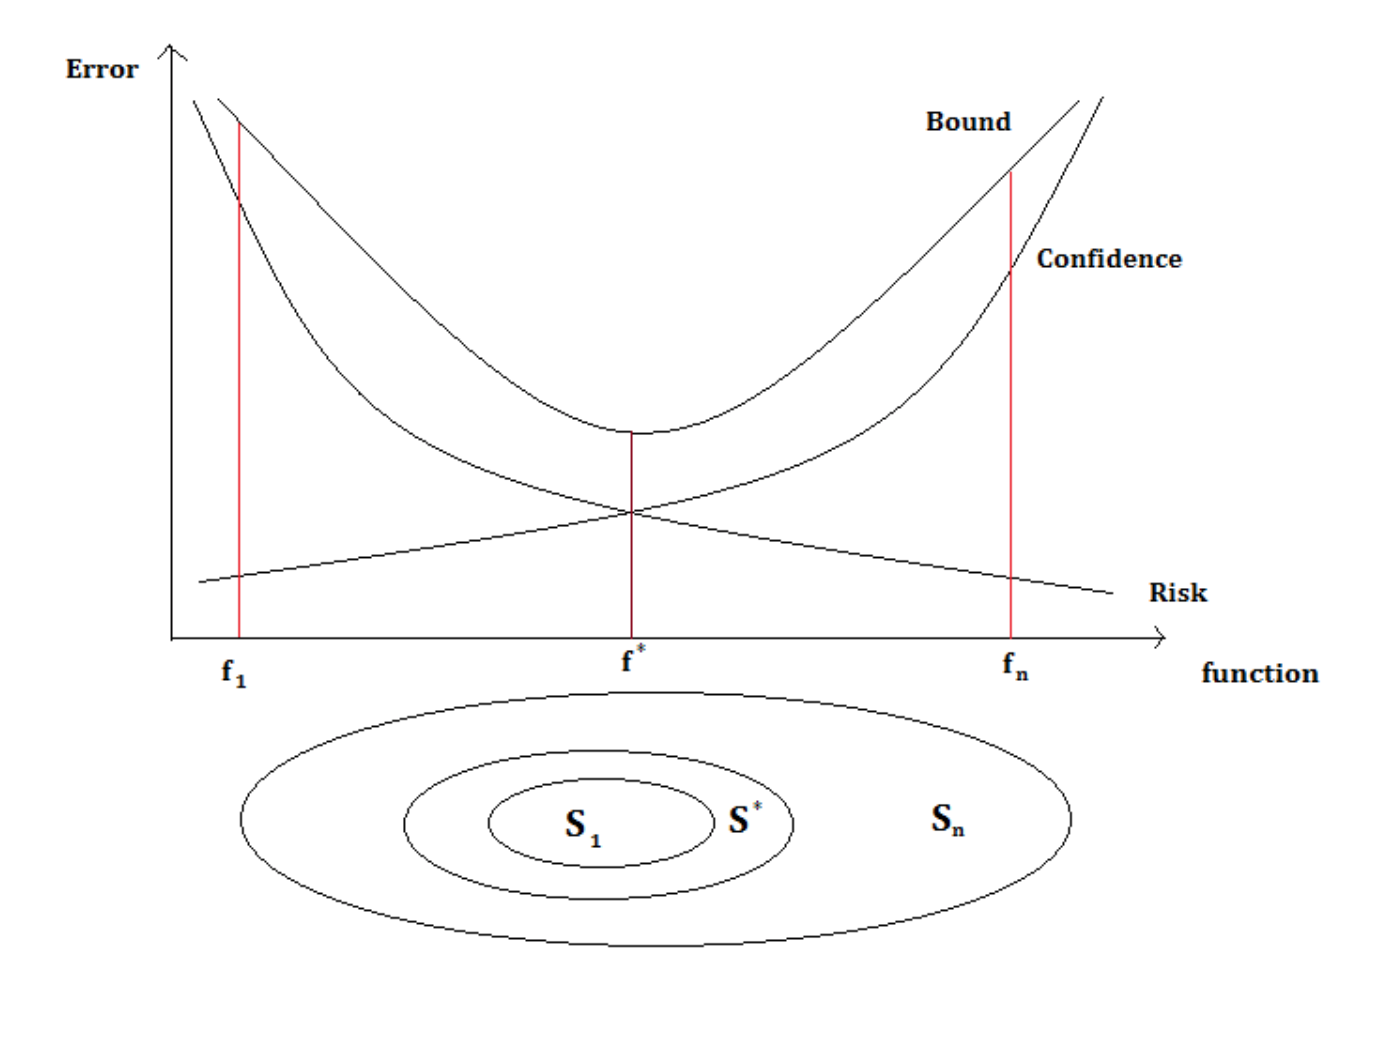
\includegraphics[scale=0.5]{SRMDiagram.png}
	\caption{An illustration of the empirical risk and confidence for different functions. The optimal function is found at the minimum of the bound, listed as $f^{*}$}
  	\label{fig:srm}
\end{figure*}

\section{Examples}


Consider a simple machine learning problem, where we need to find the ideal function to represent our model. As mentioned above, to carry out SRM we have two parts to our procedure, the first of which is finding the function $f_{i}$ that returns to us the minimum risk $R(f)$ for each structure $S_{i}$. The definition of our risk function depends on the type of problem we are solving. For a classification problem, one may want to use a zero-one loss function or a hinge-loss function. On the other hand, for a regression problem, a Huber loss function may be favourable. Once we have selected a suitable loss function, our next step is to look at functions to represent our capacity measure. The $l_{1}$-regularizer and $l_{2}$-regularizer are two examples of functions that can be used to calculate the capacity measure. 

\

Below is the formula that needs to be solved for a support vector machine, according to SRM \cite{srmneumann}:

\begin{equation}\label{srm2}
\centering
\[\underset{f}{min}\left[C\cdot\sum_{i=1}^{n}{max}\left[\left|y_{i}-f(x_{i})\right|,0\right]+\left\Vert \mathbf{w}\right\Vert _{2}^{2}\right]\]
\end{equation}

with the solution $\hat{f}(x_{i})=C_{k}\cdot K(x,x_{k})$ where $K$ represents the kernel function. Notice how SVMs use the hinge-loss function as their risk function and the $l_{2}$-regularizer to quantify complexity. 

If we are to carry this out for linear regression, our formula would
look something like this:

\begin{equation}\label{srm3}
\centering
\[\underset{f}{min}\left[\sum_{i=1}^{n}\left(f(x_{i})-y_{i}\right)^{2}+\left\Vert \mathbf{w}\right\Vert _{2}^{2}\right]\]
\end{equation}

In reality, we can use whichever regularizer we prefer, however, the $l_{2}$-regularizer has an advantage over the $l_{1}$-regularizer as it is strictly convex and differentiable everywhere.
\index{class options|)}
